\chapter{Studi Pustaka}
\section{Twitter}
Twitter adalah sebuah jaringan informasi yang terdiri dari pesan-pesan sepanjang 140 karakter yang disebut \textit{Tweet} \cite{TwitterDef:2015}. Twitter ditemukan pada tahun 2006 oleh Jack Dorsey, Evan Williams, Biz Stone, dan Noah Glass. Misi dari Twitter adalah memberikan kemampuan kepada setiap orang untuk membuat dan menyebarkan ide dan informasi secara cepat, tanpa hambatan.\\\\
Sekarang Twitter berkantor pusat di San Francisco USA. Twitter mengalami pertumbuhan yang cepat. Ditanggal 30 Juni 2015 tercatat 316 juta pengguna aktif setiap bulanya dan dalam sehari ada 500 juta tweets dikirim di seluruh dunia \cite{TwitterComp:2015}.\\\\
Pengguna Twitter di Indonesia ternyata cukup banyak. CEO Twitter Dick Costolo membeberkan bahwa jumlah pengguna Twitter di Indonesia sudah mencapai angka 50 juta dan jumlahnya makin terus bertambah \cite{TwitterUser:2015}. Selain jumlahnya yang banyak ternyata pengguna Twitter di Indonesia cukup aktif dalam menggunakan Twitter. Dalam data yang dirilis Lembaga pemantau media sosial Semiocast "Top 20 Cities by Number of posted tweets" ada dua kota di Indonesia yang masuk 10 besar kota paling aktif dalam hal tweet. Salah satunya Kota Bandung berada di posisi 5 dengan perkiraan 1.2 persen dari 10 miliar tweets selama Juni 2012.\\
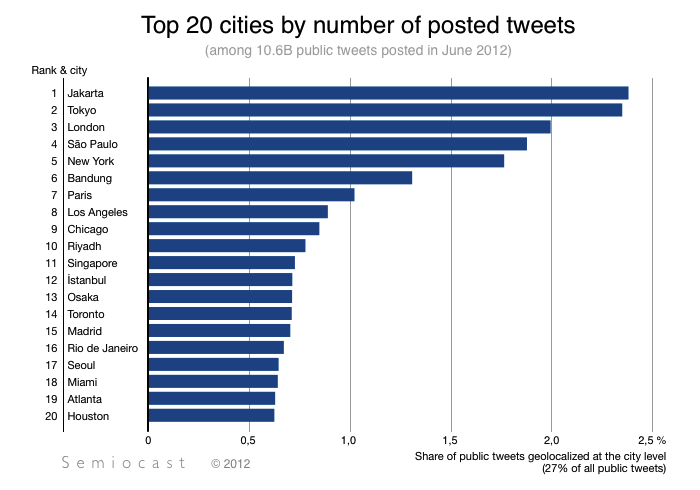
\includegraphics[width=\linewidth]{Gambar/mine/twittercity}
Tingginya popularitas Twitter dapat dimanfaatkan untuk berbagai keperluan dalam berbagai aspek, contohnya sebagai sarana komunikasi, memberikan opini, kampanye poilitik, bisnis, mendapatkan informasi, dan banyak lainya.
\section{Twitter API}
API (Application Programming Interface) merupakan sebuah cara yang didefinisikan sebuah program untuk
menyelesaikan sebuah tugas, biasanya dengan menerima atau memodifikasi data. Twitter menyediakan
sebuah API yang memberikan hak akses kepada pengembang perangkat lunak untuk membaca dan menulis data dari server Twitter. Programmer menggunakan Twitter API untuk membuat aplikasi, website, widgets, dan proyek lainya yang berinteraksi dengan Twitter. Program akan berkomunikasi dengan Twitter API melalui HTTP. Twitter menyediakan beberapa jenis dan fungsi API yang berbeda, diantaranya REST API, Streaming API, dan ads API.
\subsection{REST API}
REST API menyediakan akses secara program untuk membaca dan menulis data Twitter. Beberapa akses yang disediakan oleh Twitter seperti membuat tweet baru, membaca pro\textit{file} author and data follower, dan lain-lain. REST API mengidentifikasi aplikasi dan pengguna Twitter menggunakan OAuth. Twitter menyarankan jika pengembang berniat untuk memonitor atau memproses tweets secara real-time lebih baik menggunakan Streaming API daripada REST API, dikarenakan REST API memiliki rate limits.\\\\
Rate limiting pada API versi 1.1 ditujukan per-\textit{user} basis atau per \textit{access token}. Rate limits pada API versi 1.1 dibagi kedalam interval 15 menit. Ada 2 buah kelompok GET \textit{request} : 15 panggilan setiap 15 menit, dan 180 panggilan setiap 15 menit. Setiap endpoints membutuhkan authentication. Ini bertujuan agar mencegah kebiasaan yang buruk, dan juga dapat membantu Twitter mengerti lebih jauh bagaimana mengkategorikan aplikasi yang menggunakan API.
\subsection{Streaming API}
Streaming API memberikan latensi yang rendah kepada pengembang untuk mengakses Global Streaming Twitter dari data tweets. Pengimplementasian secara tepat dan benar dapat menghindari overhead. Twitter menawarkan beberapa streaming endpoints, setiap endpoints disesuaikan bergantung pada kasus tertentu.
\begin{enumerate}
	\item Public Streams\\
	Public Stream menyediakan data publik yang mengalir melewati Twitter. Jenis ini cocok untuk memantau spesifik \textit{user} atau topik, dan penambangan data.
	\item \textit{user} Streams\\
	\textit{user} Streams menyediakan aliran data dan spesifik kejadian untuk \textit{user} yang terautentikasi. Single-\textit{user} streams, mengandung semua data yang sesuai dengan view yang dimiliki \textit{user} tunggal dari Twitter. 
	\item Site Streams\\
	Site Streams adalah versi multi-\textit{user} dari \textit{user} streams. Site stream ditujukan untuk server yang terhubung ke Twitter atas nama banyak \textit{user}. Site streams berguna untuk menerima udates secara real-times dari jumlah \textit{user} yang banyak. 
\end{enumerate}
\subsection{Perbedaaan antara Streaming dan REST}
Streaming API dan REST API memiliki beberapa perbedaan. Karena adanya perbedaan ini, pengembang harus memikirkan jenis API mana yang cocok digunakan dalam aplikasinya. Setiap API memiliki karakteristik yang berbeda ada kelebihan yang dimiliki masing-masing API.\\\\
Ketika menggunakan Streaming API, aplikasi memerlukan koneksi HTTP yang tetap terbuka antara streaming process dengan server Twitter. Streaming API tidak dapat merespon \textit{user} \textit{request} secara langsung, namun \textit{user} \textit{request} harus ditangani oleh HTTP server yang dimiliki oleh aplikasi. Pada gambar dibawah, aplikasi memiliki 2 buah penanganan yang terdiri dari server yang menangani \textit{user} \textit{request}, dan server yang menangani streaming process.\\
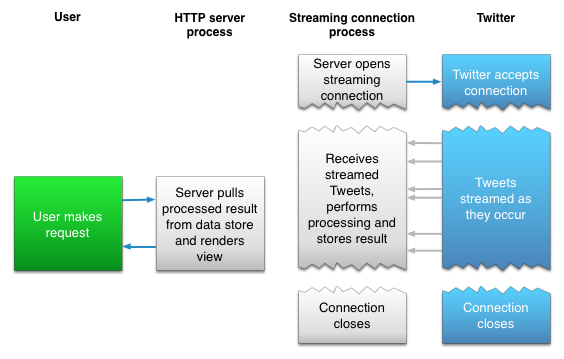
\includegraphics[width=\linewidth]{Gambar/mine/streamingapi}
Dalam menggunakan REST API aplikasi idealnya memiliki 2 buah koneksi HTTP. Koneksi \textit{user} dengan HTTP server dan Twitter server dengan HTTP server. \textit{user} \textit{request} akan diteruskan oleh HTTP server melalui REST API ke server Twitter. Respon dari server Twitter akan diproses oleh HTTP server dan diteruskan kepada \textit{user}. Gambar dibawah menggambarkan cara kerja dari REST API.\\
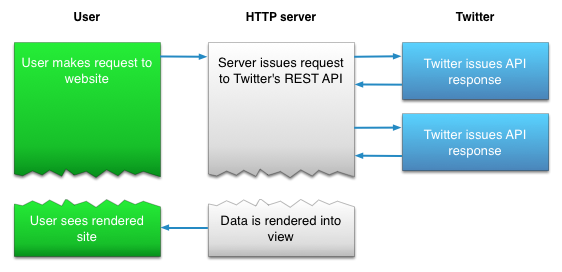
\includegraphics[width=\linewidth]{Gambar/mine/restapi}
\section{OAuth}
OAuth 2.0 authorization adalah sebuah framework yang memungkinkan sebuah aplikasi pihak ke-tiga untuk mendapatkan akses terbatas pada layanan HTTP, tanpa memberikan data autentikasi. Dalam model tradisional autentikasi \textit{client}-server, ketika \textit{client} meminta \textit{request}s sebuah akses terhadap sumber daya yang dilindungi, pemilik dari sumber daya harus memberikan surat kepercayaan kepada \textit{client}. Dalam hal mendukung aplikasi pihak ke-3, pemilik sumber daya harus membagi surat kepercayaanya kepada pihak ke-3. Hal ini menyebabkan beberapa masalah dan batasan : 
\begin{enumerate}
	\item Aplikasi pihak ke-3 perlu menyimpan surat kepercayaan pemilik sumber daya untuk penggunaan dimasa depan, biasanya adalah sebuah password dalam teks.
	\item Server perlu mendukung autentikasi password, walaupun kelemahan keamanan melekat pada passwords.
	\item Aplikasi pihak ke-3 mendapatkan seluruh akses pada sumber daya yang dilindungi. Pemilik sumber daya tidak bisa memberikan batasan akses kepada pihak ke-3.
	\item Pemilik sumber daya tidak bisa mencabut akses aplikasi pihak ke-3 tanpa mencabut seluruh akses pihak ke-3, dan harus mengganti password.
\end{enumerate}
OAuth mengatasi masalah ini dengan memperkenalkan sebuah authorization \textit{layer} dan membagi peran \textit{client} untuk mengakses sumber daya. Sebagai ganti menggunakan surat kepercayaan pemilik untuk mengakses sumber daya yang dilindungi. \textit{client} mendapatkan \textit{access token} (sebuah string yang berisi cakupan yang spesifik, waktu akses, dan attribut akses lainya.) \textit{access token} diberikan kepada \textit{client} pihak ketiga oleh authorization server dengan persetujuan pemiliki sumber daya. \textit{client} menggunakan \textit{access token} untuk mengakses sumber daya yang dilindungi oleh resource server.\\\\
Dalam OAuth didefinisikan ada 4 peran:
\begin{enumerate}
	\item Resource Owner\\
	Sebuah entitas yang dapat memberika akses kepada sumber daya yang dilindungi. Ketika resource owner seorang manusia, ini merujuk pada end-\textit{user}.
	\item Resource Server\\
	Server yang menyediakan sumber daya yang dilindungi, dapat menerima dan merespon \textit{request} sumber daya yang dilindungi menggunakan \textit{access token}s.
	\item \textit{client}\\
	Sebuah aplikasi yang meminta hak akses kepada sumber daya yang dilindungi.
	\item Authorization Server\\
	Server yang memberikan \textit{access token}s kepada \textit{client} ketika proses autentikasi berhasil.
\end{enumerate}
Protocol Flow\\
\includegraphics[width=\linewidth]{Gambar/mine/OAuth}
\begin{enumerate}
	\item \textit{client} melakukan meminta authorization grant kepada pemiliki sumber daya. \textit{request} bisa dilakukan secara langsung kepada pemilik sumber daya, atau secara tidak langsung melewati authorization server sebagai penengah.
	\item \textit{client} mendapatkan authorization grant.
	\item Authorization Grant digunakan untuk meminta \textit{access token} kepada Authorization Server.
	\item Authorization Server mengautentikasi apakah authorization grant yang dimiliki \textit{client} valid, dan jika valid, \textit{client} diberikan sebuah \textit{access token}.
	\item \textit{client} meminta sumber daya yang dilindungi dari resource Server dan melakukan autentikasi dengan memperlihatkan acces token.
	\item Resource server memvalidasi \textit{access token}, dan jika valid, server akan melayani \textit{request}.
\end{enumerate}
\section{Twitter4J}
Twitter4j adalah sebuah Java library untuk Twitter API bersifat \textit{open sourced} dan gratis. Dengan Twitter4j, \textit{user} dapat dengan mudah mengintegrasikan aplikasi Java dengan Twitter service. Twitter4j dapat di unduh pada situs twitter4j.org. Fitur yang dimiliki oleh Twitter4j antar lain :
\begin{enumerate}
	\item 100\% Java murni - bekerja pada semua platform Java versi 5 atau lebih baru.
	\item \textit{Zero dependencey} - tidak membutuhkan jars tambahan
	\item Mendukung Built-in Oauth
	\item Mendukung 100\% Twitter API 1.1
	\item Dokumentasi dengan Javadoc
\end{enumerate}
Untuk menggunakan Twitter4j disarankan mengikuti persyaratan sistem yang ditetapkan oleh pengembang Twitter4j :
\begin{enumerate}
	\item OS: Windows atau semua jenis Unix yang mendukung Java.
	\item JVM: Java 5 atau lebih baru
\end{enumerate}
Cara menggunakan Twitter4j dengan cara mengunduh jar \textit{file} Twitter4j dan menambahkan Twitter4j-core-4.0.4.jar dalam \textit{classpath} aplikasi kita. Di dalam twitter4j-core-4.0.4.jar terdapat 8 \textit{package}.
\section{Jaringan Syaraf Tiruan}
Jaringan Saraf Tiruan (JST) adalah paradigma memproses sebuah informasi yang terinspirasi dari cara kerja sistem saraf biologi, seperti otak, memproses informasi. Kunci utama dari paradigma ini adalah struktur dari sistem proses informasi. Sistem ini terdiri dari dari banyak element proses yang saling terhubung (neurons) bekerja secara serempak untuk menyelesaikan suatu masalah.  JST dikonfigurasi untuk sebuah penerapan yang spesifik, seperti  pengenalan pola atau pengklasifikasian data, melalui proses belajar. Di dalam sistem biologi belajar melibatkan penyesuaian hubungan sinaptic yang berada diantara neuron.\\\\
\subsection{Cara Kerja Jaringan Saraf Biologi}
Untuk membangun sebuah komputer yang dapat berfikir seperti manusia, para
peneiliti harus memodelkanya seperti otak manusia. Komposisi utama otak
manusia adalah sel neuron. JST harus mencoba mensimulasikan sifat-sifat dari
sel neuron itu sendiri.\\\\
Sebuah sel neuron, seperti pada gambar dibawah, menerima sinyal dari dendrit. Ketika neuron menerima sebuah sinyal, ada kemungkinan neuron tersebut meneruskan sinyal tersebut. Ketika neuron meneruskanya, sinyal tersebut ditransimisikan melewati axon neuron. Sinyal tersebut akan melewati terminal axon, dan ditransmisikan ke neuron lain.\\
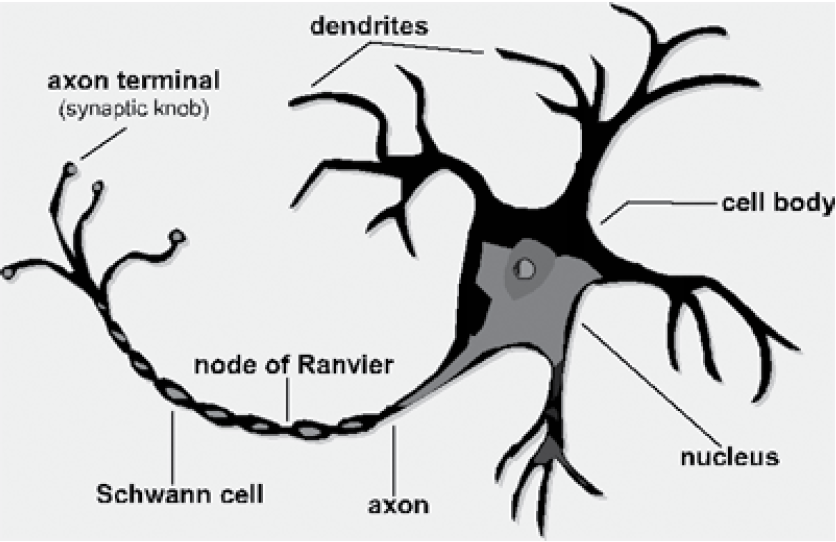
\includegraphics[width=\linewidth]{Gambar/mine/neuron}\\
\subsection{Menyelesaikan masalah dengan JST}
JST dapat memproses kumpulan informasi yang akan menghasilkan output. Output JST nantinya akan digunakan untuk membantu pengambilan sebuah keputusan. Faktanya tidak semua masalah cocok diselesaikan dengan JST. Ada beberapa jenis masalah yang kurang cocok diselesaikan oleh JST :\\
\begin{enumerate}
	\item Masalah yang dapat diselesaikan dengan program yang mudah untuk di tuliskan kedalam flowcharts.
	\item Masalah yang dapat diselesaikan dengan program yang langkahnya dapat didefnisikan dengan terperinci.
	\item Masalah yang harus diketahui cara solusinya diturunkan.
	\item Algoritma yang digunakan untuk menyelesaikan sebuah masalah tidak berubah-rubah(Statik).
\end{enumerate}
Walau tidak semua masalah dapat diselesaikan oleh JST namun ada masalah yang dapat diselesaikan secara efisien dan efektif oleh JST daripada program tradsional.\\\\
\subsection{Masalah yang dapat diselesaikan dengan JST}
Ada banyak hal yang dapat diselesaikan oleh JST. Jenis masalah yang sering diselesaikan oleh JST sebagai berikut :
\begin{enumerate}
	\item \textbf{Classification} adalah proses pengklasifikasian informasi menjadi beberapa
jenis kelompok. Contohnya, perusahaan asuransi ingin mengklasifikasikan permohononan asuransi menjadi beberapa kategori risiko yang berbeda, atau sebuah organisasi online ingin membuat sistem email mereka dapat mengklasifikasikan pesan masuk menjadi kelompok spam dan bukan spam. Untuk mencapai hal tersebut JST harus dilatih menggunakan beberapa contoh kelompok data dan instruksi. Setiap kelompok data diklasifikasikan menjadi anggota himpunan tertentu. JST dapat belajar dari contoh kelompok data tersebut. Setelah proses pembelajaran diharapkan JST dapat mengindikasi anggota kelompok data yang baru.
	\item \textbf{Prediction} adalah penerapan lain yang sering digunakan untuk JST. Dengan memberikan serangkaian input-output data berdasarkan basis waktu, sebuah JST
digunakan untuk memprediksi masa depan. Akurasi prediksi akan bergantung pada banyak faktor, seperti quantiti dan relevansi dari input data. JST biasanya diterapkan pada masalah yang melibatkan prediksi pergerakan dalam pasar finansial.
	\item \textbf{Pattern Recognition} adalah sebuah bentuk pengklasifikasian. Pattern recognition adalah kemampuan untuk mengenali pola. Pola harus bisa dikenali bahkan ketika datanya berubah. Sebagai contoh setiap pengemudi harus dapat dengan tepat mengidentifikasi lampu lalu lintas. Walaupun tidak semua lampu stopan bentuknya sama, pengemudi tetap dapat mengenalinya. Hal ini juga harus dicapai oleh JST agar komputer dapat melakukan pengenalan pola.
	\item \textbf{Optimization} suatu kemampuan JST untuk mencari solusi yang optimal. Biasanya digunakan ketika suatu masalah memiliki state space yang sangat besar. JST mungkin tidak selalu menemukan solusi optimal, namun JST dapat mencari solusi yang dapat diterima. Salah satu masalah optimasi yang paling terkenal ialah Traveling Sales Problem.
\end{enumerate}
\subsection{Metode Pembelajaran}
Ada banyak cara untuk membuat JST dapat belajar. Setiap algoritma pembelajaran nantinya akan melibatkan perubahan bobot setiap penghubung neuron. Proses pelatihan sangatlah penting bagi JST. Ada dua bentuk dari pelatihan yang dapat digunakan, supervised dan unsupervised. Pelatihan supervised melibatkan JST dengan serangkaian input-output yang diinginkan. Pelatihan unsupervised dibutuhkan juga kumpulan pelatihan, namun tidak disertai output.
\begin{enumerate}
	\item \textit{Unsupervised Training} adalah salah satu metode pembelajaran yang disediakan input data namun tidak disediakan antisipasi output. Unsupervised training biasanya digunakan untuk melatih JST klasifikasi. Penerapan lainya digunakan untuk data mining. Unsupervised training juga biasa digunakan untuk self-organizing maps (SOM). Unsupervised training dapat diterapkan kedalam banyak situasi.\\
	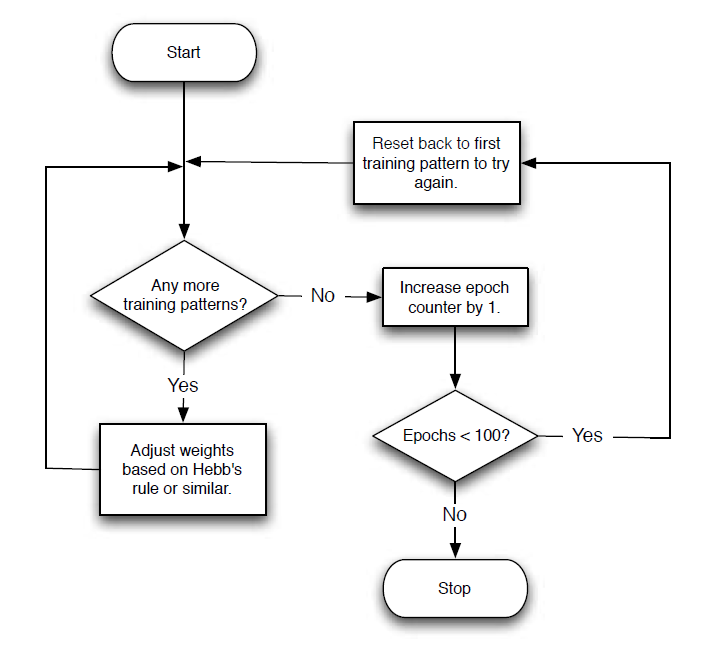
\includegraphics[width=\linewidth]{Gambar/mine/unsupervised}
	\item \textit{Supervised Training} adalah metode pembelajaran, yang memiliki sekumpulan pelatihan. Perbedaan utama antara supervised Training dan unsupervised training adalah bahwa supervised training disediakan outputs harapan. Hal ini memungkinkan JST untuk menyesuaikan
nilai dari bobot matrix berdasarkan perbedaan antara output yang diharapkan dengan output yang sesunguhnya.\\
	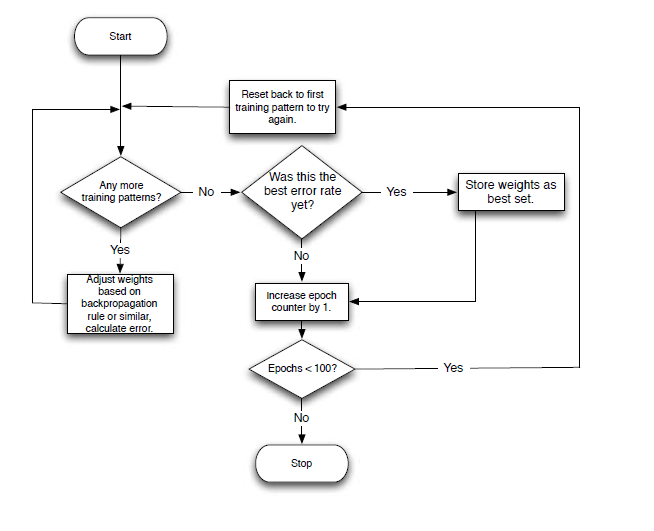
\includegraphics[width=\linewidth]{Gambar/mine/supervised}
\end{enumerate}
\subsection{Perhitungan Galat}
Perhitungan galat adalah salah satu aspek penting dari setiap JST. Apakah JST itu adalah supervised atau unsupervised, sebuah rata-rata galat harus dihitung. Tujuan dari setiap algoritma pelatihan ialah untuk meminimalisasi rata-rata galat.
\subsubsection{Perhitungan Galat dan Supervised Training}
Ada dua nilai yang harus dipertimbangkan dalam menentukan rata-rata galat untuk supervised training. Pertama kita harus menghitung galat untuk setiap element pelatihan. Kedua, kita harus menghitung rata-rata galat untuk semua element pelatihan untuk setiap sampel. (Root Mean Square) RMS adalah salah satu metode untuk menghitung rata-rata galat untuk sebuah pelatihan. Metode RMS efektif dalam perhitungan rata-rata galat tanpa memperhatikan apakah hasil yang sebenarnya lebih tinggi atau lebih kecil daripada hasil yang diharapkan. Persamaan ini digunakan untuk menghitung RMS\\\\
$ x_{rms}= \sqrt{\frac{1}{n}\sum_{i=1}^{n}(actual_{i}-ideal_{i})^2} $\\\\
\section{Feedforward Neural Network}
Feedforward adalah sebuah arsitektur JST yang paling popular dan paling banyak digunakan sebagai model dalam banyak penerapan. Feedforward dikenal juga sebagai "multi-layer perceptron." Dalam JST feedforward, setiap layer dari JST mengandung hubungan ke layer berikutnya (contohnya dari input dihubungkan ke layer tersembunyi). Hubungan antar neuron pada feedforward hanya satu arah. Feedfoward selalu dimulai dari layer input. Jika input terhubung dengan sebuah layer tersembunyi, layer tersembunyi dapat terhubung dengan layer tersembunyi lainya atau dapat langsung terhubung dengan output. Jumlah layer tersembunyi bisa banyak. Kebanyakan JST biasanya akan memiliki satu buah layer tersembunyi, dan akan sangat jarang JST memiliki lebih dari dua buah layer tersembunyi.
\subsection{Memilih Struktur Jaringan}
Ada banyak cara untuk membangun JST feedforward. Kita harus menentukan berapa jumlah neuron pada layer input dan layer output. Selain itu layer tersembunyi harus ditentukan. Ada banyak teknik untuk memilih parameter tersebut. Namun untuk menentukan struktur yang optimal pada feedforward dibutuhkan pengalaman dan percobaan.
\begin{itemize}
\item\textbf{Layer Input} \\Jumlah neuron pada layer input dapat ditentukan bergantung pada data yang kita miliki. Parameter ini biasanya ditentukan secara unik ketika kita mengetahui data pelatihan kita. Secara spesifik, jumlah dari neuron setara dengan banyaknya kolum pada data kita. Biasanya kita dapat menambahkan satu buah titik bias.
\item\textbf{Layer Output} \\Seperti input layer, setiap JST memiliki satu buah layer output. Untuk jumlah neuron di dalamanya ditentukan pada model apa yang kita gunakan. Apakah JST kita Machine Mode atau Regression Mode. Machine Mode mengembalikan label kelas, sedangkan Regression Mode mengembalikan sebuah nilai. bila JST menggunakan sebuah regressor, maka outputnya akan memiliki 1 neuron. Bila outputnya sebuah pengklasifikasian, maka neuronya akan satu atau lebih.
\item\textbf{Layer Tersembunyi}\\Dalam layer tersembunyi ada dua buah keputusan yang harus diperhatikan. Pertama menentukan berapa jumlah layer tersembunyi yang dibutuhkan. Kedua menentukan berapa jumlah  neuron pada setiap layer.\\\\ 
Secara teori tidak ada alasan untuk menggunakan layer tersembunyi lebih dari dua. Faktanya pada masalah yang ada pada kehidupan sehari-hari, cukup diselesaikan dengan 1 buah layer tersembunyi. Tabel berikut merupakan kegunaan JST berdasarkan banyaknya layer tersembunyi\\\\
\begin{tabular}{|l|p{7cm}|}
\hline
Number of Hidden Layer & Result \\\hline
none & Only capable of representing linear separable functions or decisions.\\\hline
1 & Can approximate any function that contains a continuous mapping from one finite space to another.\\\hline
2 & Can represent an arbitrary decision boundary to arbitrary accuracy with rational activation functions and can approximate any smooth mapping to any accuracy.\\\hline
\end{tabular}\\\\
Untuk menentukan jumlah neuron dalam layer tersembunyi adalah bagian yang sangat penting dalam menentukan keseluruhan arsitektur JST. Walaupun layer ini tidak secara langsung berinteraksi dengan lingkungan luar, layer ini memiliki pengaruh yang sangat besar pada akhir output. Jumlah layer tersembunyi dan jumlah neuronya sangat penting diperhatikan. Jika kita terlalu sedikit menggunakan neuron dalam layer tersembunyi ini akan mengakibatkan sesuatu yang disebut underfitting. Namun bila terlalu banyak menggunakan neuron pada layer tersembunyi ini akan mengakibatkan overfitting. Overfitting terjadi ketika JST terlalu banyak memiliki informasi yang diproses daripada jumlah batas dari informasi yang terkandung dalam sejumlah pelatihan. Ada beberapa tips untuk menentukan jumlah neuron: Pertama jumlah neuron harus berada diantara jumlah input dan output. Kedua jumlah neuron seharusnya 2/3 ukuran dari layer input, ditambah dengan layer output. Ketiga jumlah neuron seharusnya kurang dari dua kali dari layer input.
\item\textbf{Fungsi Aktivasi}\\
Kebanyakakn JST mengeluarkan output dari layernya menggunakan fungsi aktivasi. Fungsi aktivasi ini menskalakan output dari JST dalam jangkauan tertentu. Fungsi aktivasi dapat kita buat sendiri namun umumnya menggunakan fungsi yang sudah sering digunakan. Ada beberapa jenis fungsi aktivasi yang sering digunakan diantara sebagai berikut:
\textbf{Sigmoid} adalah fungsi aktivasi yang menggunakan fungsi sigmoid untuk menentukan aktivasi. fungsi sigmoid di definisikan sebagai berikut:\\\\
$f(x)=\frac{1}{1+e^{-x}}$\\\\
Kurva dibawah menggambarkan fungsi sigmoid\\\\
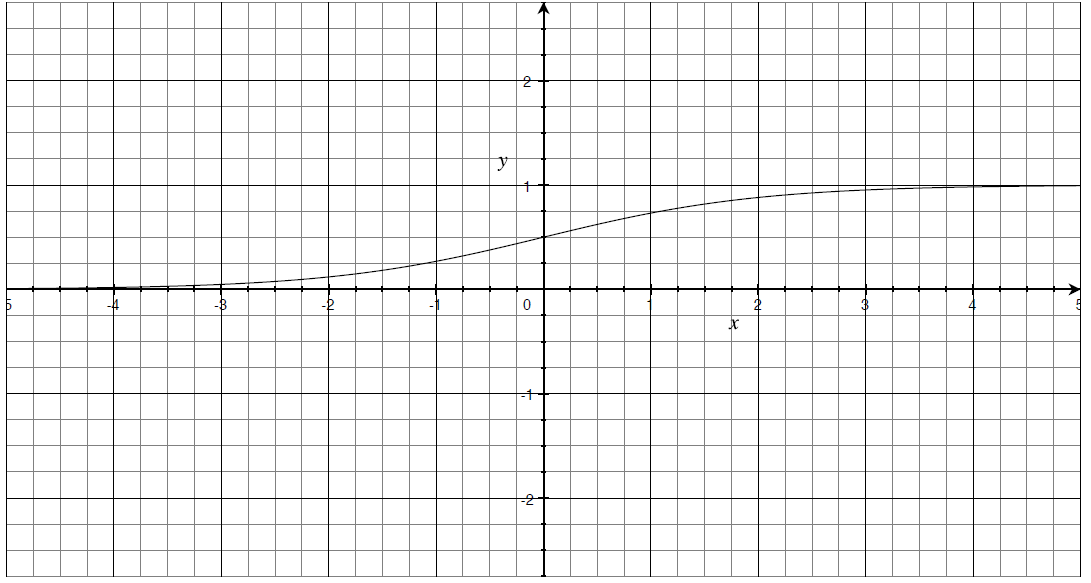
\includegraphics[width=\linewidth]{Gambar/mine/sigmoid}
Hal penting yang perlu diperhatikan dalam menggunakan fungsi sigmoid. Fungsi ini hanya akan menghasilkan nilai positif.
\textbf{Hyperbolic Tangent}
berbeda dengan sigmoid bila pada sigmoid selalu menghasilkan nilai positif. Dengan menggunakan fungsi Hyperbolic Tangent akan menghasilkan nilai negatif. Bila kita menginginkan output dapat bernilai negatif dan positif kita dapat menggunakan fungsi yang di definisikan sebagai berikut:\\\\
$f(x)=\frac{e^{2x}-1}{e^{2x}+1}$\\\\
Kurva dibawah menggambarkan fungsi Hyperbolic Tangent\\\\
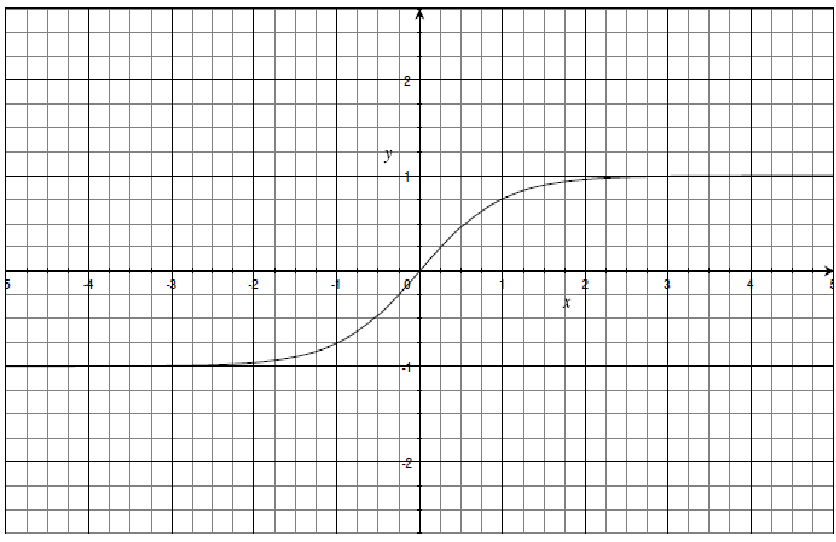
\includegraphics[width=\linewidth]{Gambar/mine/tangent}
\end{itemize}
